\documentclass[11pt,a4paper]{article}
\usepackage[margin=2.2cm]{geometry}
\usepackage{amsmath,amssymb,bm}
\usepackage{graphicx}
\usepackage{booktabs}
\usepackage[hidelinks]{hyperref}
\usepackage{natbib}
\graphicspath{{figures/}}
\newcommand{\apj}{ApJ}\newcommand{\apjl}{ApJL}\newcommand{\mnras}{MNRAS}\newcommand{\aap}{A\&A}\newcommand{\jcap}{JCAP}\newcommand{\prd}{Phys.\ Rev.\ D}\newcommand{\aj}{AJ}\newcommand{\apjs}{ApJS}\newcommand{\physrep}{Phys.\ Rep.}
\newcommand{\dF}{\delta_F}
\newcommand{\kl}{\kappa_{{\rm Ly}\alpha}}
\newcommand{\kc}{\kappa_{\rm CMB}}
\newcommand{\vl}{\bm{L}}
\newcommand{\vth}{\bm{\theta}}
\newcommand{\Mpch}{\,h^{-1}{\rm Mpc}}
\title{Weak lensing of the DESI DR1 Lyman-$\alpha$ forest by low-redshift galaxies and quasars:\\ estimator, validation and a first amplitude constraint}
\author{An\v{z}e Slosar (with Claude)}
\date{15 September 2026}
\begin{document}
\maketitle

\begin{abstract}
Gravitational lensing by structure at $z<2$ displaces the Lyman-$\alpha$ forest sightlines coherently, which dilates and shears the transverse correlation of the forest flux. We measure this effect with a pair-based quadratic estimator: the products of forest pixels on pairs of sightlines are weighted by the response of the measured forest correlation to a deflection and projected on a template of the lensing deflection built from DESI DR1 galaxies and quasars at $0.4<z<1.75$ (LRG, ELG and QSO samples in five redshift slices). The tracer template shares no density modes with the forest at $2.1<z<3$, so unlike a CMB-lensing template it is free of the intrinsic forest--density three-point term that we found to bias the CMB cross-correlation at the $0.4$ level of the lensing amplitude. On 400 self-lensed mock realisations with lognormal tracers the estimator is unbiased (null $-0.05\pm0.08$, recovery $0.91\pm0.08$, paired response $0.966\pm0.025$ for a true amplitude of one). Applied to 373\,756 DR1 forests over $11\,000\,{\rm deg}^2$ and templates whose linear biases are measured from their own angular power spectra and cross-checked against ACT DR6 CMB lensing, the lensing amplitude relative to the $\Lambda$CDM prediction is $A=-0.10\pm0.75$ (single slab), i.e. $A<1.14$ at 95 per cent, with curl, random-template and injection tests consistent with no systematic. A detection at this depth was not expected; the full DESI sample should reach $2$--$3\sigma$.
\end{abstract}

\section{Summary}
This note documents the measurement in a self-contained way: the data (Section~\ref{sec:data}), the estimator and its templates (Section~\ref{sec:estimator}), the mock validation that defines its acceptance (Section~\ref{sec:mock}), the DR1 result with its null tests (Section~\ref{sec:result}) and the caveats (Section~\ref{sec:caveats}). The derivations of the estimator and the CMB-lensing forecasts are in the project's main report (\texttt{report/main.pdf}); the pipeline is \texttt{code/pipeline} (mocks, estimator, campaign) and \texttt{code/stageb} (DR1). Every number quoted here is in the committed JSON products under \texttt{report/}.

\section{Data}
\label{sec:data}
\paragraph{Forest.} The DESI DR1 Lyman-$\alpha$ forest deltas \citep{2503.14745,2306.06312}: 428\,403 forests extracted with \texttt{picca} v9 over $1040$--$1205$\,\AA\ rest frame on a 0.8\,\AA\ grid, with the lines, DLA (combined CNN + Gaussian-process catalogue, $N_{\rm HI}>10^{20.3}\,{\rm cm}^{-2}$) and BAL masks applied by the DR1 extraction. We keep pixels with $2.1\le z\le3.0$ and forests with at least 50 such pixels: 373\,756 forests, $1.8\times10^8$ pixels, 11\,013\,deg$^2$ (nside-64 pixels containing a forest), a median of 471 pixels per forest. Pixel weights are the \texttt{picca} weights $w=1/(\eta\sigma_N^2+\sigma^2_{\rm LSS}(\lambda))$ with $\eta\simeq1$ and $\sigma^2_{\rm LSS}=0.07$--$0.19$: the diagonal of the inverse covariance, including the signal variance. The per-forest noise power $P_N=\sigma_N^2\Delta\chi_{\rm pix}$ has median $0.54\Mpch$ and a scatter of 2.2 in $\ln P_N$.

\paragraph{Tracers.} The DR1 large-scale-structure clustering catalogues v1.5 \citep{2405.16593}: LRG ($0.4<z<1.1$), ELG\_LOPnotqso ($0.8<z<1.6$) and QSO ($z<1.75$ here), with their completeness, redshift-failure and imaging-systematics weights, and two random catalogues per Galactic cap (5000\,deg$^{-2}$) carrying redshifts and weights. They are split into five redshift slices, $0.4$--$0.6$, $0.6$--$0.8$ (LRG), $0.8$--$1.1$ (LRG, ELG, QSO), $1.1$--$1.6$ (ELG, QSO) and $1.6$--$1.75$ (QSO), all in front of the forest box ($z<1.8$). Figure~\ref{fig:kernel} shows where they sit under the lensing kernel of a source at $z=2.4$: the five slices contain $69$--$77$ per cent of the power of $\kl$ (the forest's own slab contributes 0.5 per cent; $z<0.4$ the rest).

\paragraph{CMB lensing.} The ACT DR6 baseline convergence \citep{2304.05203,2304.05202} is used only to cross-check the tracer biases (Section~\ref{sec:templates}).

\begin{figure}
\centering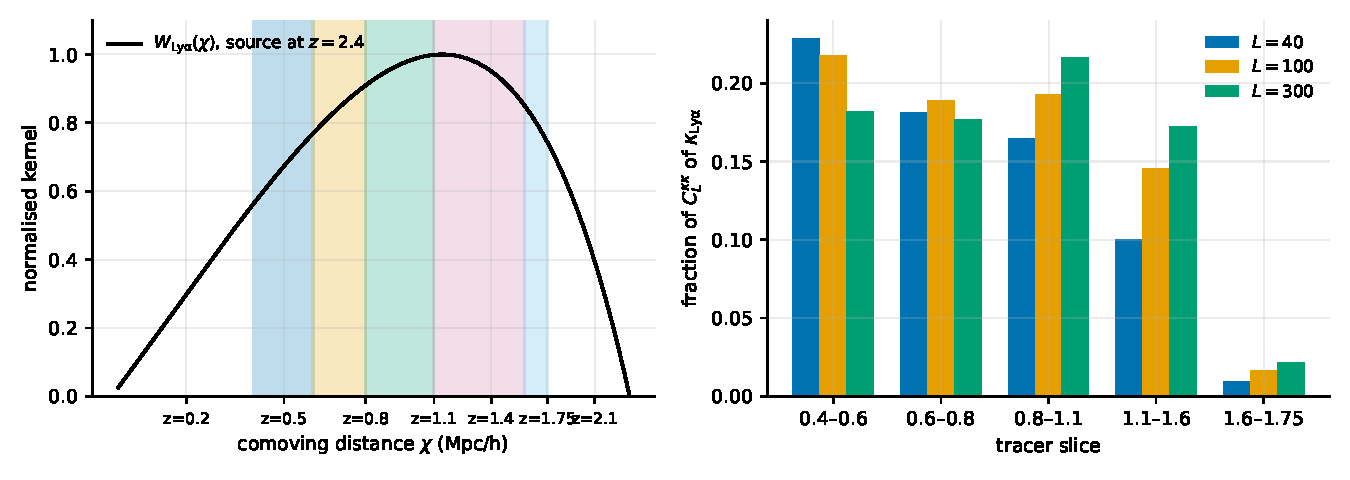
\includegraphics[width=\textwidth]{kernel_slices.pdf}
\caption{Left: the lensing kernel of a source at $z=2.4$ (the effective forest redshift) with the five tracer slices shaded. Right: the fraction of the power of $\kl$ contributed by each slice at $L=40$, 100 and 300 (Limber, non-linear matter power); the slices together hold 69--77 per cent.}
\label{fig:kernel}
\end{figure}

\section{Estimator}
\label{sec:estimator}
\subsection{Lensing of pair correlations}
Let $\dF(\vth,\chi)$ be the forest flux fluctuation observed along a sightline at angular position $\vth$ and comoving distance $\chi$. Lensing maps the observed position to the true one, $\vth_{\rm true}=\vth+\bm\alpha(\vth)$, with $\bm\alpha=\nabla\phi$ and $\kappa=-\nabla^2\phi/2$, so that the observed field is the true field sampled at $\vth+\bm\alpha$. For a pair of sightlines $a,b$ the correlation of two pixels at transverse separation $r_\perp=\chi|\vth_a-\vth_b|$ and radial separation $r_\parallel$ is the true correlation at the displaced separation,
\begin{equation}
\langle\dF(a,\chi_p)\dF(b,\chi_q)\rangle=\xi_F\!\left(\bigl|\vth_{ab}+\bm\alpha_a-\bm\alpha_b\bigr|\chi,\,r_\parallel\right)
\simeq\xi_F(r_\perp,r_\parallel)+\frac{\partial\xi_F}{\partial r_\perp}\,\chi\,\hat\vth_{ab}\cdot(\bm\alpha_a-\bm\alpha_b),
\label{eq:pair}
\end{equation}
with $\hat\vth_{ab}$ the unit pair direction (from $b$ to $a$). For a pair separation small compared with the wavelength of the lens, $\bm\alpha_a-\bm\alpha_b\simeq(\vth_{ab}\cdot\nabla)\nabla\phi$: the convergence dilates the transverse correlation isotropically and the shear makes it anisotropic. Equation~\eqref{eq:pair} is exact in the pair displacement and does not require the squeezed limit; the deflection difference is evaluated from the template at the two sightlines.

\subsection{Quadratic estimator with a deflection template}
\label{sec:qe}
Given a template deflection $\bm\alpha^T(\vth)$ for the lensing field, the amplitude $A$ of the deflection in the data ($\bm\alpha=A\,\bm\alpha^T$ in expectation) is estimated from all pixel pairs on all sightline pairs with $3\le r_\perp\le30\Mpch$ and $|r_\parallel|<30\Mpch$,
\begin{equation}
\hat A=F^{-1}(q-\bar q),\qquad
q=\sum_{ab}\;\bigl[\chi_{ab}\,\hat\vth_{ab}\cdot(\bm\alpha^T_a-\bm\alpha^T_b)\bigr]\sum_{p\in a,q\in b}w_pw_q\,\dF(p)\dF(q)\,\xi'_F(r_\perp,r_\parallel),
\label{eq:qe}
\end{equation}
with $\xi'_F=\partial\xi_F/\partial r_\perp$ the response kernel, $\bar q$ the mean field (the same sum with $\dF(p)\dF(q)$ replaced by $\xi_F$: it removes the correlation of the sightline density with the template and is not zero on a masked footprint), and $F$ the response matrix, $\sum w_pw_q\,\xi'^2_F\,[\chi\hat\vth\cdot\Delta\bm\alpha^T]^2$ up to the same geometric factors. This is the optimal quadratic estimator for the pixel-diagonal inverse covariance; a full per-sightline inverse covariance would shape the weights along $k_\parallel$ and we estimate its gain at 8 per cent in signal-to-noise, not worth its complexity here. The pair geometry uses a local tangent-plane metric per pair, valid at the separations used; the sightline density is 19--22\,deg$^{-2}$ so the pair count is $3.9\times10^6$.

The template deflection is split into three multipole bands, $40\le L<100$, $100$--$200$ and $200$--$300$ (cosine-tapered windows), plus the complementary ``junk'' band, and each band has a curl partner (the deflection rotated by $90^\circ$). The seven components are fitted jointly with the $7\times7$ response matrix; the science amplitude is the common amplitude of the three gradient bands with the curl and junk amplitudes marginalised (a ``curl null'' is reported as the mean curl amplitude). Errors are from a HEALPix jackknife on the pair midpoints (nside 8, 301 regions on DR1) and are checked against the Fisher scale $F^{-1/2}$ and against random templates.

\paragraph{The response kernel.} $\xi_F(r_\perp,r_\parallel)$ is measured from the same forests in 1\,$\Mpch$ cells and fitted with the model
\begin{equation}
\xi_F(r_\perp,r_\parallel)=\xi_{\rm ref}(r_\perp,r_\parallel;b_F^2,\beta_F)+\sigma(r)\,S(r_\perp,r_\parallel)+N(r_\perp)\,\mathbb{1}[\,|r_\parallel|<1\Mpch\,],
\label{eq:xifit}
\end{equation}
where $\xi_{\rm ref}$ is the two-parameter linear model $P_F(\bm k)=b_F^2(1+\beta_F\mu^2)^2P(k)$ pushed through the DESI pixel and resolution windows and the per-forest continuum operator; $S$ is a tensor-product cubic B-spline in $(r_\perp,r_\parallel)$ carried on a strictly positive envelope $\sigma(r)$, $r=(r_\perp^2+r_\parallel^2)^{1/2}$ (the monopole of $\xi_{\rm ref}$), which removes the dynamic range of $\xi_F$ from the spline coefficients; and $N$ is a one-dimensional spline confined to the first radial bin. Every basis element is averaged over the 1\,$\Mpch$ cell exactly as the pair counts are binned, and all 50 parameters are fitted by weighted least squares with the accumulated pair weights, so that $\xi_F$ and its \emph{analytic} derivative $\xi'_F$ follow the data rather than a two-parameter shape. Three points matter.

\emph{(i) Why the shape has to be fitted.} The estimator normalisation is $\langle\hat A\rangle=A\,\langle Wg_{\rm used}g_{\rm true}\rangle/\langle Wg_{\rm used}^2\rangle$ with $g=\chi\,\xi'_F$ and $W$ the pair weight, so an error in the \emph{shape} of the kernel biases the amplitude at first order; it does not cancel. The two-parameter table misses the DR1 measurement by 5--12 per cent at $r_\parallel<5\Mpch$, which is where 80 per cent of the information is, and its free three-coefficient version returns $\beta_F=0.43$ from the $\mu^2$ term against $\beta_F=1.76$ from the $\mu^4$ term: the Kaiser form itself is rejected. Fitting the correction changes $\chi^2$ from 1880 to 235 over 810 cells and raises the amplitude normalisation by 8 per cent.

\emph{(ii) The continuum projection.} The correlation the pixels see is $P_aCP_b^\mathsf{T}$ with $P_a$ the mean-and-slope removal of the continuum fit on forest $a$; it is the largest single distortion of the model. Earlier iterations evaluated it for one representative forest spanning the whole slab (1295 pixels, $712\Mpch$) with uniform weights, while the median picca forest has 689 pixels ($397\Mpch$); that over-predicted $\xi_F$ by 5--20 per cent, growing with $r_\perp$. It is now the pair-weight average of $P_aCP_b^\mathsf{T}$ over sampled pairs of real DR1 forests, with the measured pixel weights and with the projector running over every pixel the continuum fit saw (not only the pixels inside $2.1<z<3.0$). The corrected projection removes the mean offset but predicts more $r_\perp$ tilt than the data show, which is why the empirical correction is still needed.

\emph{(iii) The same-wavelength term.} Pixels at the same observed wavelength on different sightlines carry an extra positive correlation of $\simeq10^{-3}$, flat in $r_\perp$ beyond $6\Mpch$ and significant at 5--7$\sigma$ per cell, absent from the neighbouring radial bins (Figure~\ref{fig:xicorr}): a sky-subtraction and calibration residual, not a correlation of the density field. It therefore belongs in the mean field, which subtracts $\langle\dF\dF\rangle$, but carries no lensing response, and $N$ is excluded from $\xi'_F$ for that reason.

On DR1 the fit gives $b_F^2=0.0300$ and $\beta_F=1.02$ over $3\le r_\perp<30$, $r_\parallel<30\Mpch$ (Figure~\ref{fig:xi}); the base parameters are not measurements of the forest bias, since the correction absorbs part of the shape. Non-linear Arinyo-i-Prats terms were tested and make the fit \emph{worse} at these separations, monotonically in $q_1$ ($\chi^2=1249,1300,1357,1421$ for $q_1=0,0.3,0.6,0.9$ with the old projection), while $k_p$ is degenerate with the pixel window; this is consistent with the DESI DR1 full-shape analysis, which bounds $q_1<0.51$ at 95 per cent from the same data and leaves $\{k_v,a_v,b_v,k_p\}$ prior-dominated, and which fits the auto-correlation only at $r>25\Mpch$ \citep{2509.15308}. The lensing information is concentrated at small radial separations: 80 per cent of it comes from $r_\parallel<5\Mpch$ and half from $r_\perp<15\Mpch$ (Figure~\ref{fig:profile}).

\emph{How much freedom to give the correction.} The correction is fitted to the same pixel pairs that the estimator multiplies, so a random error $\delta g$ in the kernel attenuates the amplitude by $\langle W\,{\rm Var}(\delta g)\rangle/\langle Wg^2\rangle$: more parameters buy a better fit and cost response. Both sides are measurable. On DR1 the amplitude gain saturates almost at once --- $1.077$ with one cubic segment in each direction (16 coefficients for $S$ plus 6 for $N$), $1.099$ with 30, $1.100$ with 42 --- while the cost, measured on 40 mock realisations in Section~\ref{sec:mock}, does not: the paired response falls by $1.4\pm1.2$, $4.0\pm1.8$ and $10.4\pm2.3$ per cent for the same three. We therefore adopt the smallest, a bicubic surface in $(r_\perp,r_\parallel^2)$ with 22 fitted parameters in all, which takes $\chi^2$ from 1880 to 235 over the 810 cells and costs no measurable response.

\emph{Robustness.} With that choice the fitted kernel is insensitive to the parts of the construction that are choices rather than data. Across four continuum-projection variants (single full-slab forest; pair-weighted with the redshift-cut span; pair-weighted with the full picca span; an independent Monte-Carlo sample of the latter) the amplitude normalisation lies between $1.075$ and $1.079$ and the Fisher-weighted kernels agree to 2.0--5.3 per cent rms. We adopt the full-picca-span projection and quote $1.077$ for the normalisation change, with a 2 per cent systematic covering the knot and projection variations.

\begin{figure}
\centering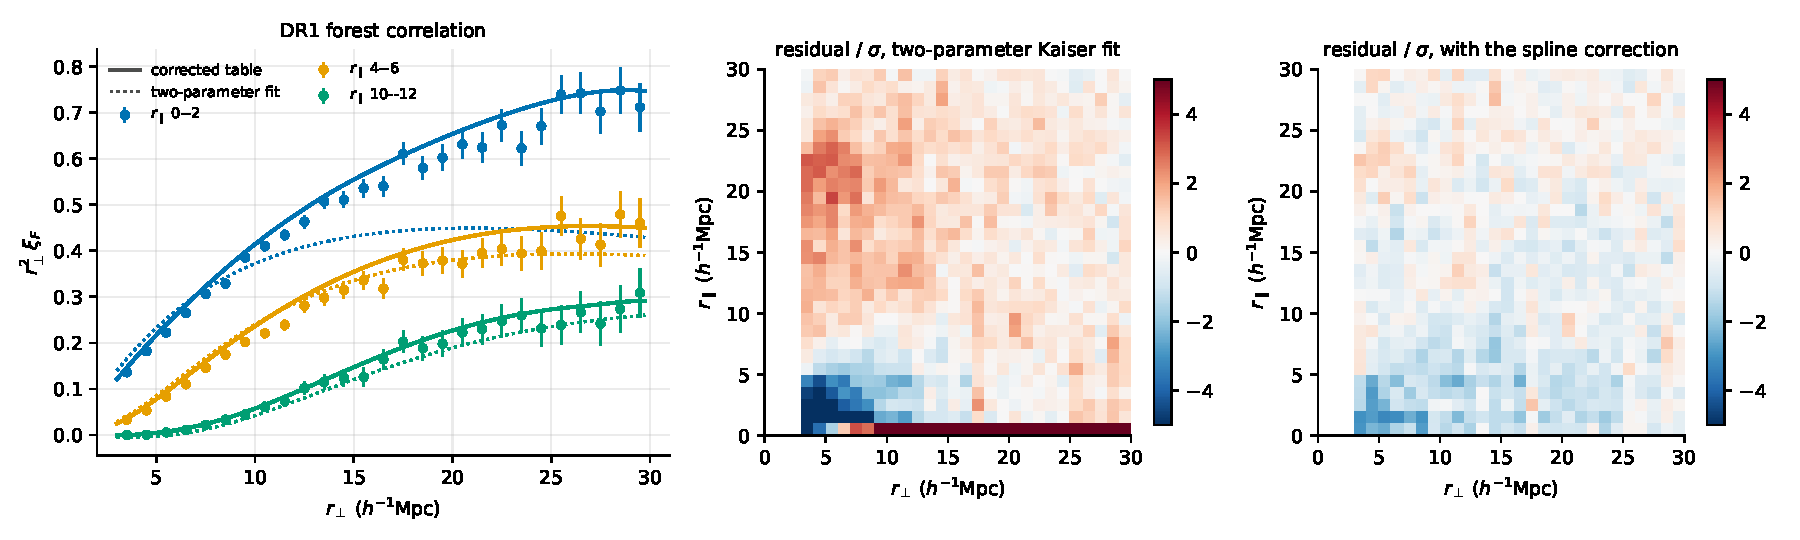
\includegraphics[width=\textwidth]{dr1_xi.pdf}
\caption{DR1 forest correlation from $1.8\times10^8$ pixels. Left: measured $r_\perp^2\xi_F$ in three radial-separation strips (points, pair-weight errors) with the fitted table of Equation~\eqref{eq:xifit} (solid) and the two-parameter Kaiser fit of the same counts and basis (dotted). Middle and right: the residual of each fit in units of the per-cell error, on the $(r_\perp,r_\parallel)$ plane used by the kernel. The two-parameter fit is systematically high at $1<r_\parallel<5\Mpch$, where most of the lensing information is, and low by up to a factor 1.6 in the first radial bin; $\chi^2$ over the 810 fitted cells falls from 1880 to 235.}
\label{fig:xi}
\end{figure}

\begin{figure}
\centering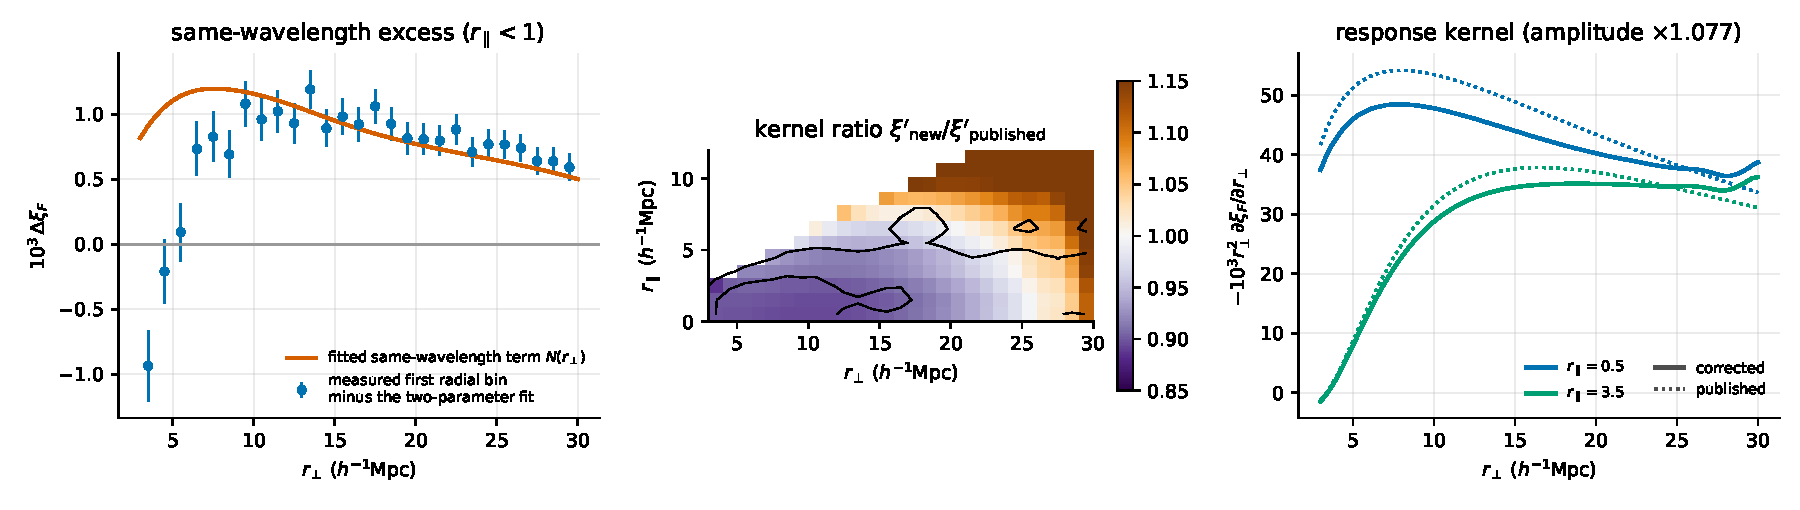
\includegraphics[width=\textwidth]{xi_correction.pdf}
\caption{What the correction does. Left: the excess of the first radial bin over the two-parameter fit (points) and the fitted same-wavelength term $N(r_\perp)$ (line); it is flat at $\simeq10^{-3}$ beyond $6\Mpch$ and enters the mean field but not the kernel. Middle: the ratio of the new response kernel to the one used in the first measurement, over the part of the pair domain where the kernel is large, with contours of the Fisher-information density of the amplitude. Right: the kernel itself, $-r_\perp^2\,\partial\xi_F/\partial r_\perp$, at two radial separations, published (dotted) against corrected (solid). Fisher-weighted, the kernel change raises the lensing amplitude by 10 per cent.}
\label{fig:xicorr}
\end{figure}

\begin{figure}
\centering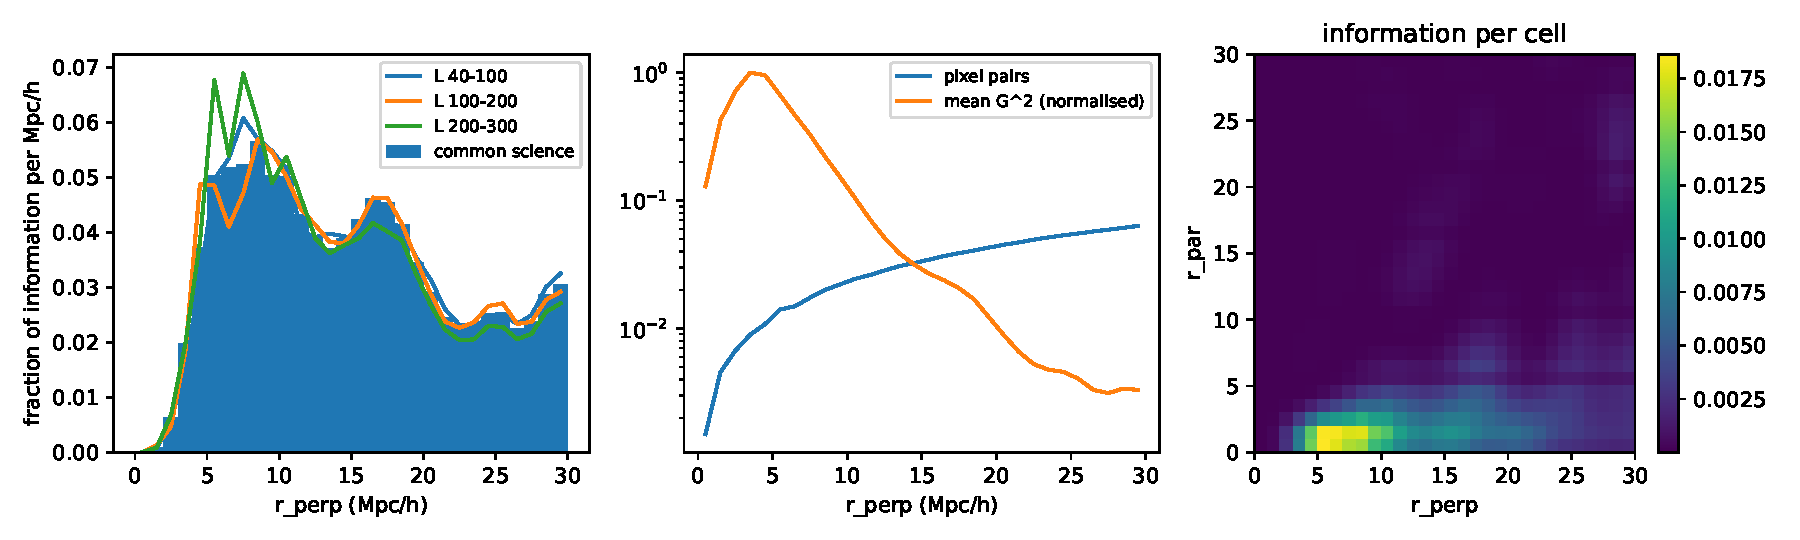
\includegraphics[width=.8\textwidth]{signal_profile.pdf}
\caption{Where the lensing information lives: the cumulative Fisher information of the amplitude versus $r_\perp$ and $r_\parallel$ on a scale-1 mock, per band and combined. Half of the information is inside $r_\perp=15\Mpch$ and 80 per cent at $r_\parallel<5\Mpch$.}
\label{fig:profile}
\end{figure}

\subsection{Templates from low-redshift tracers}
\label{sec:templates}
For a tracer with objects at $(\vth_i,\chi_i)$ and mean density $\bar n(\chi)$ per steradian per unit distance, the kernel-weighted map
\begin{equation}
m(\vth)=\sum_{i\in{\rm pixel}}\frac{w_i\,W(\chi_i)}{b\,\bar n(\chi_i)\,\Omega_{\rm pix}}-\text{(randoms, scaled)},\qquad W(\chi)=\frac{3}{2}\Omega_m\frac{H_0^2}{c^2}(1+z)\chi\frac{\chi_s-\chi}{\chi_s},
\end{equation}
estimates the contribution of the tracer's slice to $\kl$ for a source at $\chi_s=\chi(2.4)$, once the linear bias $b$ of the tracer is known: $\langle m\rangle=\int_{\rm slice}W\delta\,d\chi$. The randoms define the footprint (pixels holding at least half the mean random count, which excludes partially covered rim pixels), the completeness (their density smoothed by $1^\circ$) and the mean-density subtraction; the map is built at nside 512.

\paragraph{Bias from the angular power spectrum.} The bias of every (tracer, slice) is measured from its own map: the cross-spectrum of two random halves of the catalogue (which has no shot noise) is fitted against the Limber spectrum of the slice, $C_\ell=b^2\int_{\rm slice}W^2P(k=(\ell+\tfrac12)/\chi,\chi)\,d\chi/\chi^2$, times the pixel window and a Monte-Carlo transfer of the survey mask (0.8--0.9 in the band for the fragmented DR1 footprint), on large scales only, $40\le\ell\le0.2\,\chi(z_{\rm mid})$ ($k\le0.2\,h\,{\rm Mpc}^{-1}$), with Gaussian bandpower errors. The shot noise of the full map is measured from the half difference and agrees with the weighted Poisson expectation $\sum_i(u_iw_i)^2\Omega_{\rm pix}^2/\Omega_{\rm mask}$ to 1--3 per cent for the LRG and ELG samples (plain $1/\bar n$ is 20--34 per cent too low because the weights enter squared). Figure~\ref{fig:spectra} shows the spectra and Table~\ref{tab:bias} the biases.

\begin{figure}
\centering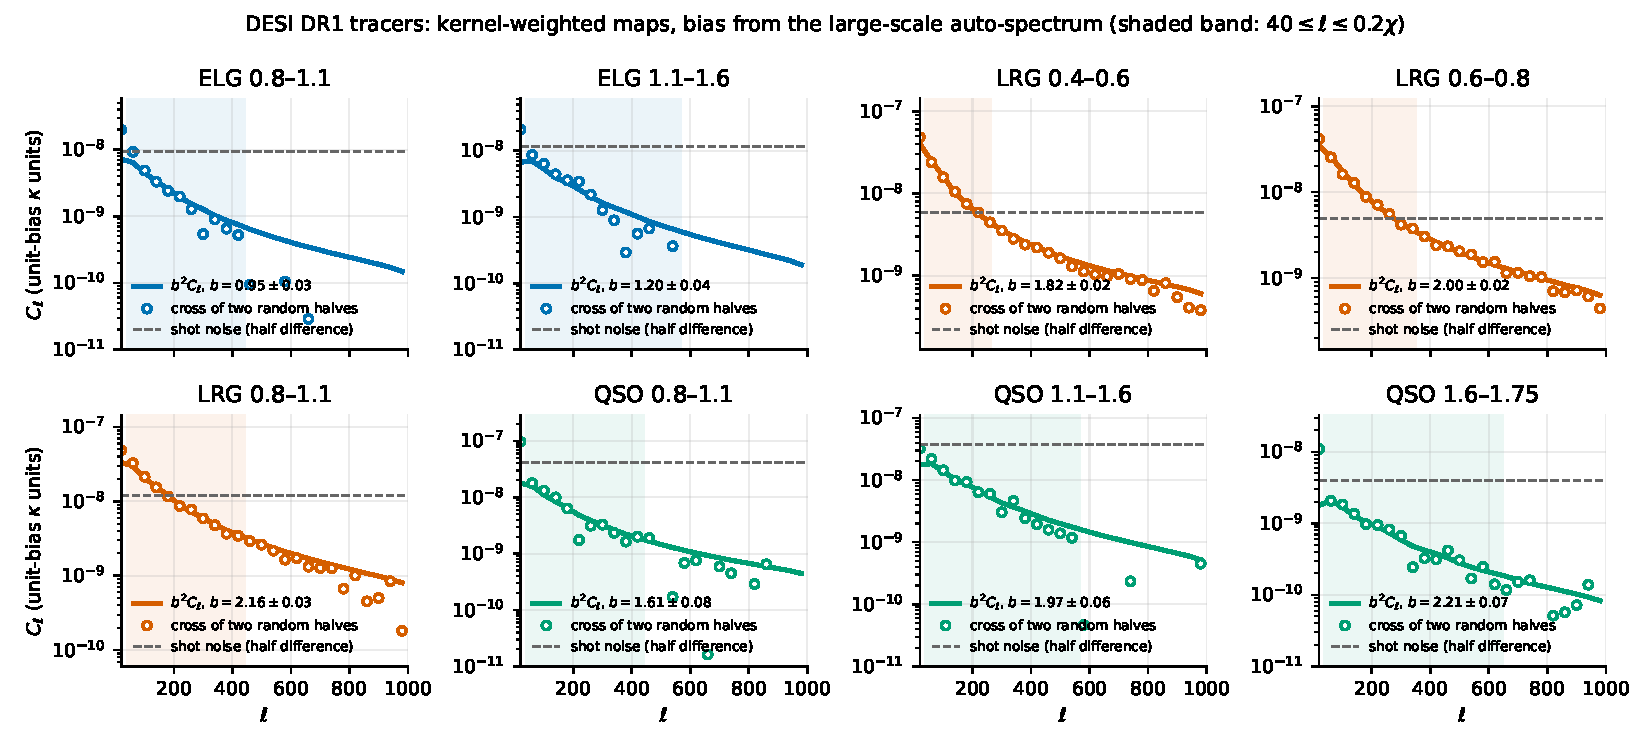
\includegraphics[width=\textwidth]{tracer_spectra.pdf}
\caption{Angular power spectra of the eight DR1 tracer maps in convergence units for unit bias: the cross-spectrum of two random halves (points, no shot noise), the fitted $b^2C_\ell$ (line) and the shot noise measured from the half difference (dashed). The shaded band is the fit range $40\le\ell\le0.2\chi(z_{\rm mid})$.}
\label{fig:spectra}
\end{figure}

\paragraph{Cross-check with CMB lensing.} The cross-spectrum of each unit-bias map with the ACT DR6 convergence map on their overlap (joint sky fraction 0.05--0.08; ACT mask squared on the $\kappa$ side as the release prescribes; $f_{\rm sky}$ scaling) gives $b$ from $\langle m\kc\rangle=b\int_{\rm slice}W\,W_{\rm CMB}P\,d\chi/\chi^2$ without any shot-noise model (Figure~\ref{fig:cmb}, Table~\ref{tab:bias}). Every slice is detected in cross-correlation at 5--13$\sigma$; six of the eight biases agree with the auto-spectrum values within 1--2$\sigma$ (10--17 per cent), while the ELG and QSO of the $0.8$--$1.1$ slice are 40 per cent lower in the cross (2.9$\sigma$ each), the ELG auto-spectrum also showing the falling $b(\ell)$ characteristic of residual imaging systematics. The templates use the auto-spectrum biases.

\begin{table}
\centering\small
\begin{tabular}{lrrrrr}
\toprule
tracer, slice & objects & $b$ (auto-spectrum) & $b$ (ACT $\kappa$ cross) & ratio & $b$ (literature)\\
\midrule
LRG 0.4--0.6 & 506\,911 & $1.82\pm0.02$ & $1.50\pm0.20$ & 0.83 & $\sim$1.9\\
LRG 0.6--0.8 & 771\,894 & $2.00\pm0.02$ & $2.04\pm0.18$ & 1.02 & $\sim$2.1\\
LRG 0.8--1.1 & 859\,822 & $2.17\pm0.03$ & $2.35\pm0.17$ & 1.08 & $\sim$2.3\\
ELG 0.8--1.1 & 1\,016\,365 & $0.96\pm0.03$ & $0.58\pm0.13$ & 0.60 & $\sim$1.3\\
ELG 1.1--1.6 & 1\,415\,707 & $1.20\pm0.04$ & $1.12\pm0.14$ & 0.93 & $\sim$1.4\\
QSO 0.8--1.1 & 143\,846 & $1.61\pm0.08$ & $0.95\pm0.23$ & 0.59 & 1.7\\
QSO 1.1--1.6 & 358\,775 & $1.97\pm0.06$ & $2.14\pm0.20$ & 1.09 & 2.1\\
QSO 1.6--1.75 & 115\,295 & $2.22\pm0.07$ & $2.02\pm0.40$ & 0.91 & 2.5\\
\bottomrule
\end{tabular}
\caption{Linear biases of the DR1 tracer slices from their large-scale auto-spectra (split-catalogue cross-spectrum, $40\le\ell\le0.2\chi$) and from the cross-spectrum with the ACT DR6 lensing map; the last column gives the DESI clustering values and, for the quasars, $b_{\rm QSO}(z)=0.278[(1+z)^2-6.565]+2.393$ at the slice centre, as orientation.}
\label{tab:bias}
\end{table}

\begin{figure}
\centering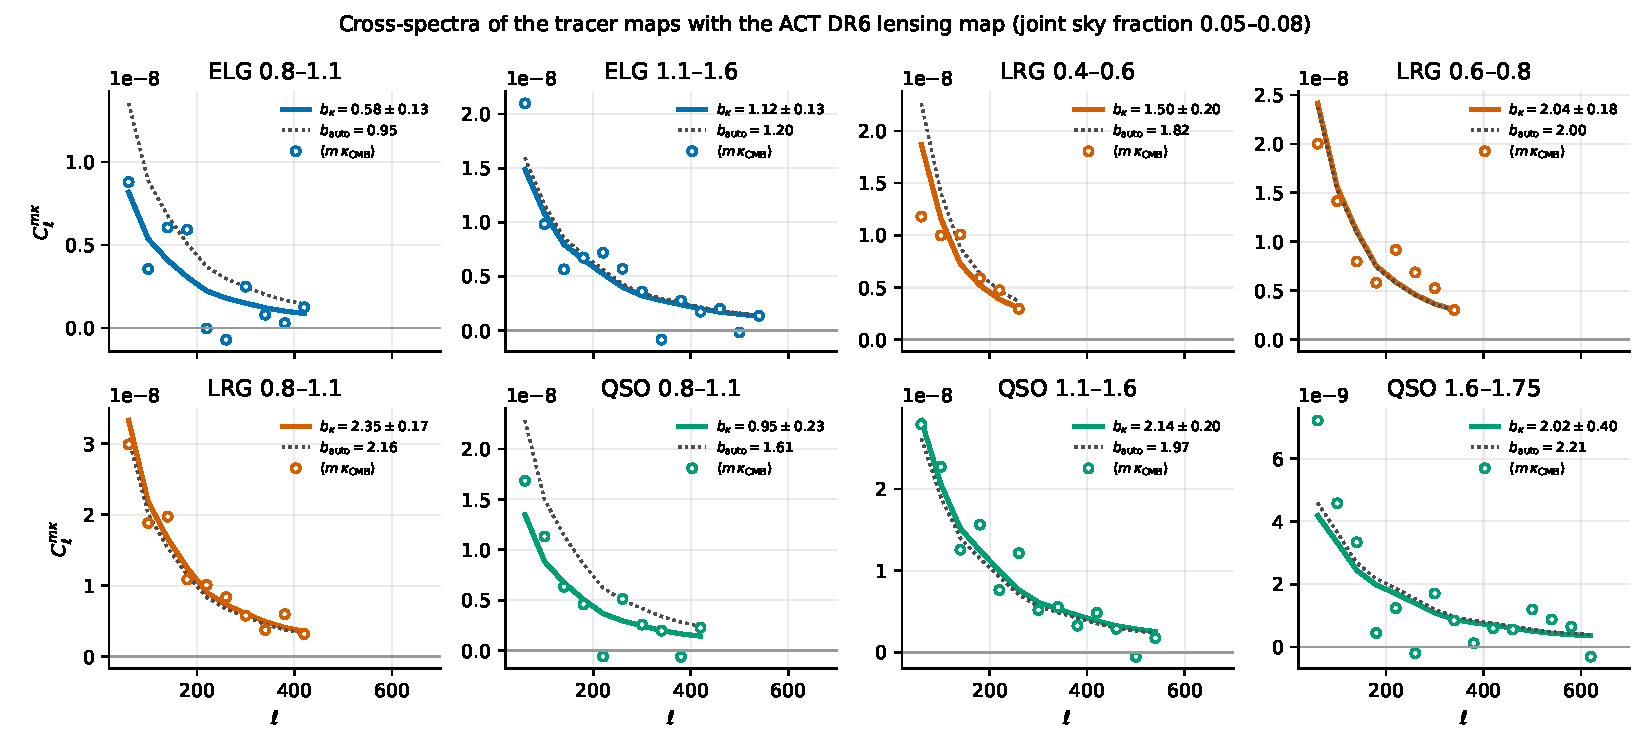
\includegraphics[width=\textwidth]{cmb_cross.pdf}
\caption{Cross-spectra of the unit-bias tracer maps with the ACT DR6 lensing map (points) with the theory scaled by the cross-correlation bias (solid) and by the auto-spectrum bias (dotted).}
\label{fig:cmb}
\end{figure}

\begin{figure}
\centering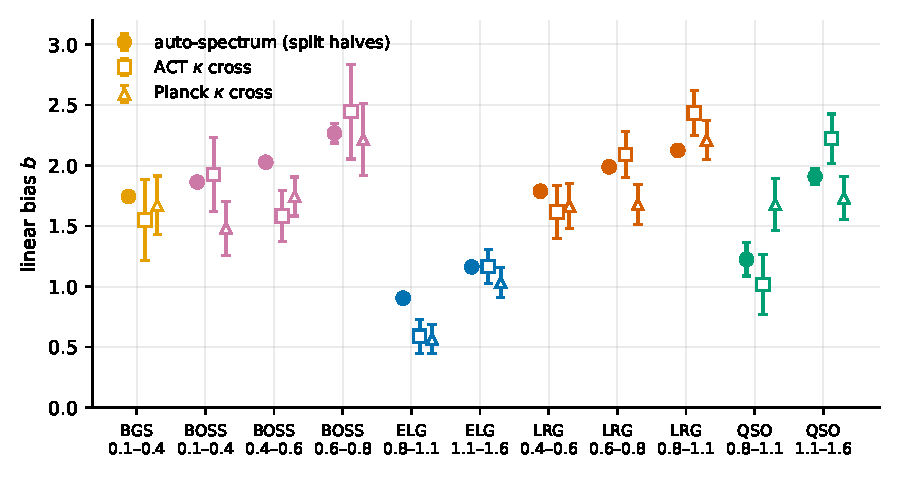
\includegraphics[width=.7\textwidth]{biases.pdf}
\caption{The two bias estimates of Table~\ref{tab:bias}.}
\label{fig:biases}
\end{figure}

\paragraph{Wiener combination and the deflection template.} Within a slice the tracer maps (in convergence units, $m/\hat b$) are combined with the weights $\bm w_\ell=\mathsf C_\ell^{-1}\bm s_\ell$ of the model covariance $\mathsf C_{kl}=S_\ell+N_k\delta_{kl}$ ($S_\ell$ the slice's convergence spectrum, $N_k$ the measured shot noise): inverse-shot-noise weighting of the tracers, Wiener-suppressed where noise dominates. The slices are independent, so the sum of the filtered slice maps is the conditional expectation of $\kl$ given all tracers; its deflection, $\bm\alpha^T=\nabla\phi$ with $\phi_{LM}=2\kappa_{LM}/[L(L+1)]$, evaluated at the sightlines (\texttt{healpy} derivatives at nside 512), is the combined template. Because the filter is the conditional-expectation coefficient, the amplitude estimator of Section~\ref{sec:qe} is normalised to $A=1$ for the true lensing without further calibration; each slice is also fitted on its own and the five slice amplitudes are combined with their joint jackknife covariance as a cross-check.

\subsection{Why not a CMB-lensing template}
The same estimator cross-correlated with $\kc$ measures lensing plus the intrinsic forest--forest--density three-point function of the forest's own redshift range. Its linear part, the response of the small-scale forest power to long-wavelength modes, can be removed with a kernel-matched template built from the $z>2$ quasars (the ``deprojection'' of the main report), but the second-order part, $\langle m_pm_qT\rangle$ with $m$ the long-wavelength component of the forest and $T$ a non-Gaussian tracer template, cannot be removed by one coefficient: on 400 mock realisations it biased the deprojected amplitude by $-0.41\pm0.18$ with no lensing and no response present. The lensing signal, the response and this term all act through the same long modes at the pair separations used, so the term has to be modelled, not filtered. A tracer at $z<1.8$ shares no density modes with the forest at $z>2.1$: its correlation with the pair products is lensing only, plus the magnification of the sightline quasars (absorbed by the mean field) and shared sky systematics.

\section{Validation on mocks}
\label{sec:mock}
The mocks are flat-sky FFT realisations of a $20^\circ\times20^\circ$ patch: a Gaussian matter field on a 2\,$\Mpch$ grid over the forest box $2.1<z<3.0$ (plus margins) from which the forest is a linear, redshift-space-distorted filter with $b_F=-0.13$, $\beta_F=1.6$ and a small-scale cut-off; 22 sightlines per deg$^2$ with pixel noise $P_N=0.33\Mpch$ (log-normal scatter across forests) and per-forest continuum projection; the ACT DR6 mask cut-out and a smooth completeness pattern; lognormal quasars behind the slab draw the sightlines. The foreground of $\kl$ (and of $\kc$) is generated in the five tracer slices as Gaussian projected-density maps with the exact Limber covariance between the density and the two convergence contributions, plus the uncovered rest; each slice hosts 2-D lognormal Poisson tracers of the projected density smoothed transversely by 3\,$\Mpch$ (a lognormal of the raw 0.7\,$\Mpch$ cells is absurdly non-Gaussian), with DR1-like biases and densities. The forest is lensed by the full $\kl$ (sampling at the displaced positions), and every realisation carries both a lensed and an unlensed forest.

The protocol (\texttt{GATES.md} v7) was frozen before the scale-1 campaign: 400 fresh realisations, templates built from each realisation's own tracers exactly as on the data (bias from the auto-spectrum, Wiener combination, sum over slices), and the gate ``an unbiased detection against a lognormal redshift tracer''. Figure~\ref{fig:mock} and Table~\ref{tab:mock} give the result: the combined null and recovery are unbiased, the paired response (the same realisation lensed and unlensed, free of sample variance) is $0.966\pm0.025$, equal to the response of the truth template ($0.970\pm0.018$; the 3 per cent deficit of the noisy sparse sample was already seen with the CMB template and is a property of the noisy forest, not of the template chain), the per-slice responses are unity within errors, a template from another realisation gives zero, the curl is zero, the jackknife error matches the ensemble scatter, and the noise-free injection expectation (the bookkeeping test of signs, cuts and band basis) has odd slope $0.98$. The only rows of the protocol that fail are the tracer-bias precision rows: the auto-spectrum bias of a lognormal tracer differs from the generator's by 1--3 per cent, resolved at $N=400$ against a 2-SEM rule that amounts to 0.4 per cent; the effect on $A$ is the same 1--3 per cent per slice.

\begin{figure}
\centering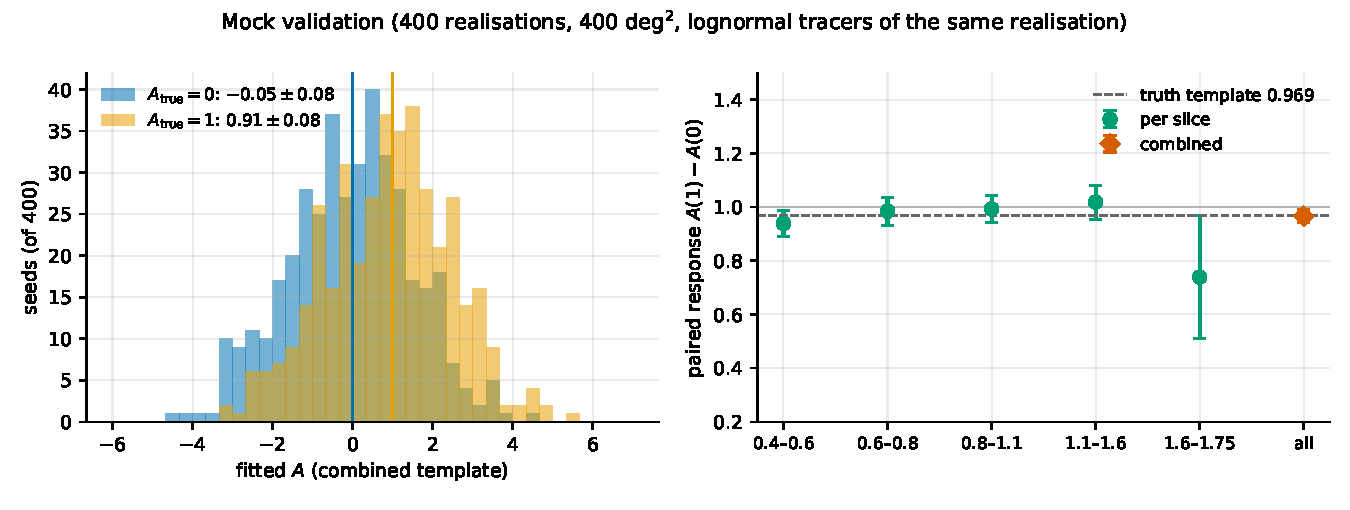
\includegraphics[width=\textwidth]{mock_validation.pdf}
\caption{Mock validation on 400 realisations. Left: the combined-template amplitude for an unlensed ($A_{\rm true}=0$) and a lensed ($A_{\rm true}=1$) forest of the same realisations. Right: the paired response $A(1)-A(0)$ per slice and combined, against the truth template.}
\label{fig:mock}
\end{figure}

\paragraph{What the corrected response table costs.} The acceptance campaign above was run with the two-parameter table of iteration 5. The correction of Equation~\eqref{eq:xifit} is fitted to the same pixel pairs the estimator weights, so it can only lose response, never gain it, on a mock whose model shape is already correct. Forty of the 400 realisations were refitted with each variant of the correction and with the two-parameter table, everything else identical (\texttt{code/pipeline/validate\_xi\_correction.py}, \texttt{report/xi\_correction\_mocks\_variants.json}); the paired responses are

\begin{center}\small
\begin{tabular}{lrrrr}
\toprule
response table & fitted parameters & paired response & ratio & DR1 amplitude gain\\
\midrule
two-parameter (iteration 5) & 2 & $0.974\pm0.071$ & --- & 1\\
\textbf{bicubic correction (adopted)} & \textbf{22} & $\mathbf{0.988\pm0.073}$ & $\mathbf{1.014\pm0.012}$ & \textbf{1.077}\\
medium knots & 36 & $0.935\pm0.068$ & $0.960\pm0.018$ & 1.099\\
fine knots & 48 & $0.873\pm0.064$ & $0.896\pm0.023$ & 1.100\\
fine knots, no same-wavelength term & 42 & $0.900\pm0.066$ & $0.924\pm0.022$ & 1.067\\
\bottomrule
\end{tabular}
\end{center}

\noindent The ratios are paired differences on the same realisations, so their errors are much smaller than those of the responses themselves. They follow the attenuation $\langle W\,{\rm Var}(\delta g)\rangle/\langle Wg^2\rangle$ computed from the least-squares covariance of the fit, which gives 0.7, 2.4 and 4.1 per cent for the three knot sets on the same mock: the right ordering, and about $2.5$ times smaller than measured, the difference being the correlation between neighbouring cells that the diagonal pair weights ignore. The adopted correction costs nothing measurable, and the same calculation on the DR1 counts gives 0.25 per cent before that factor. The mock forests carry no sky residual, so the same-wavelength term has nothing real to fit there; that it is not the source of the attenuation is visible in the last row, which removes it and recovers only a third of the loss.

\begin{table}
\centering\footnotesize
\begin{tabular}{lll}
\toprule
statistic (400 realisations, 400\,deg$^2$) & value & requirement\\
\midrule
combined null, $A_{\rm true}=0$ & $-0.05\pm0.08$ & $\le2$\,SEM; 95\% bound 0.21 ($\le0.5$)\\
combined recovery, $A_{\rm true}=1$ & $0.91\pm0.08$ & $\le2$\,SEM; 95\% bound 0.24 ($\le0.5$)\\
paired response $A(1)-A(0)$ & $0.966\pm0.025$ & $|\,\cdot-1|\le2$\,SEM\\
truth-template paired response & $0.970\pm0.018$ & report\\
per-slice responses (0.4--0.6 \ldots 1.6--1.75) & $0.94,0.99,0.99,1.02\ (\pm0.05)$; $0.74\pm0.23$ & each within 2\,SEM\\
other-realisation template & $0.01\pm0.08$ & $|\,\cdot\,|\le2$\,SEM\\
curl (combined) & $-0.07\pm0.10$ & $|\,\cdot\,|\le2$\,SEM\\
scatter / RMS jackknife & 0.96 & 0.7--1.3\\
normalisation slope on $A\in\{0,\tfrac12,1,2\}$ & $0.97\pm0.06$ & within 2\,SEM of 1\\
response on $-$ off & $0.08\pm0.09$ & $|\,\cdot\,|\le2$\,SEM\\
injection expectation, odd slope at $|A|=0.25$ & 0.980 & $1\pm0.05$\\
tracer biases $b_{\rm fit}/b_{\rm true}$ & 0.97--1.01 ($\pm0.002$--$0.004$) & 2\,SEM (fails for 6 of 8)\\
per-seed scatter of the combined amplitude & 1.56 & (CMB deprojected estimator: 3.7)\\
\bottomrule
\end{tabular}
\caption{Iteration-7 acceptance (\texttt{report/lowz\_validation.md}).}
\label{tab:mock}
\end{table}

\section{Measurement on DR1}
\label{sec:result}
The full run (one Perlmutter node, 25 minutes, 16\,GB) fits the forest correlation, builds the pair catalogue ($3.9\times10^6$ sightline pairs), evaluates the five slice templates and the combined template at the 373\,756 sightlines, and fits the seven-component basis. Table~\ref{tab:dr1} and Figure~\ref{fig:dr1} give the result:
\begin{equation}
A=-0.10\pm0.75\ \text{(combined template, jackknife; Fisher scale 0.65)},\quad A<1.14\ \text{at 95 per cent (one-sided)}.
\end{equation}
The five slices are individually consistent with zero and their jackknife-covariance combination, $-0.08\pm0.72$, agrees with the combined template (the slice correlations are below 0.08). The nulls: the curl amplitude is $-0.20\pm1.96$; forty Gaussian random realisations of the combined map's own spectrum through the tracer mask, fitted exactly like the data, give a mean of $-0.12\pm0.12$ and a scatter of 0.73 against the RMS jackknife error 0.81 (the jackknife is 11 per cent conservative).

\paragraph{Effect of the refined kernel.} With the two-parameter table of Section~\ref{sec:qe} the same run gives $A=0.01\pm0.67$. The error moves by the factor $1.077$ that the Fisher-weighted kernel change predicts (the Fisher scale, $0.601\to0.646$, follows it exactly); the shift of the central value, $-0.11$ in $A$ or $0.15\sigma$, is the part of the change that is not a rescaling, namely the kernel shape and the same-wavelength contribution to the mean field. The noise-free injection expectation moves from $1.014$ to $1.038$, and that is a property of the test rather than of the estimator: the injection displaces the whole table, including the same-wavelength term, which the kernel deliberately omits because it is not lensed. Repeating the injection with that term removed from the injected correlation returns $1.014$ (\texttt{report/stageb/injection\_same\_wavelength\_v3.json}), so the bookkeeping of signs, cuts and the band basis is unchanged.

\begin{table}
\centering\small
\begin{tabular}{lrrrr}
\toprule
template & $A$ & jackknife & Fisher & curl\\
\midrule
combined (five slices) & $\mathbf{-0.101}$ & $\mathbf{0.754}$ & 0.646 & $-0.20\pm1.96$\\
slice 0.4--0.6 & $-0.84$ & 1.23 & 1.21 & $-2.6\pm3.7$\\
slice 0.6--0.8 & $-0.59$ & 1.53 & 1.16 & $1.8\pm3.5$\\
slice 0.8--1.1 & $1.43$ & 1.31 & 1.19 & $2.9\pm3.7$\\
slice 1.1--1.6 & $-1.25$ & 1.95 & 1.78 & $-6.1\pm5.2$\\
slice 1.6--1.75 & $6.5$ & 6.8 & 6.5 & $-9\pm20$\\
jackknife combination of the slices & $-0.082$ & 0.715 & & \\
random templates (40) & $-0.12\pm0.12$ & scatter 0.73 & RMS jackknife 0.81 & \\
\midrule
combined, two-parameter table & $0.010$ & $0.670$ & 0.601 & $-0.18\pm1.79$\\
\bottomrule
\end{tabular}
\caption{DR1 lensing amplitude, single slab $2.1<z<3.0$, with the corrected response table (\texttt{report/stageb/dr1\_lowz\_v3.md}); the last row is the first measurement, with the two-parameter table.}
\label{tab:dr1}
\end{table}

\begin{figure}
\centering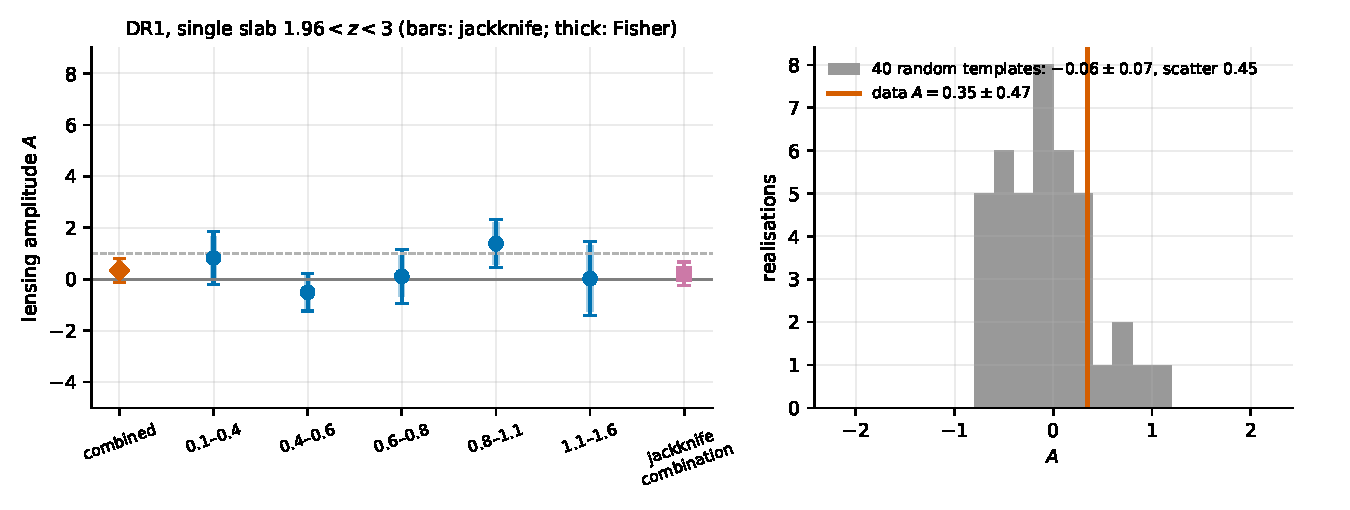
\includegraphics[width=\textwidth]{dr1_result.pdf}
\caption{Left: the DR1 amplitudes per slice and combined (thin bars: jackknife, thick: Fisher) and the jackknife-covariance combination of the slices; the dashed line is the $\Lambda$CDM value. Right: the forty random-template amplitudes with the data value.}
\label{fig:dr1}
\end{figure}

\section{Caveats and systematics}
\label{sec:caveats}
At an error of 0.75 on $A$, systematic effects of 20 per cent are irrelevant; the following are recorded for the full-DESI measurement.
\begin{itemize}
\item \emph{Tracer biases.} The auto-spectrum and CMB-cross biases agree to 10--17 per cent for six tracers; the ELG and QSO of the $0.8$--$1.1$ slice disagree by 40 per cent. A bias error $f$ scales that slice's amplitude by $1/f$; with the slice weights the combined amplitude moves by a few per cent. The ELG auto-spectrum has a scale-dependent bias above $\ell\simeq300$ (imaging systematics).
\item \emph{Forest correlation model.} The correction of Equation~\eqref{eq:xifit} is empirical: it is fitted to the same pixel pairs that the estimator multiplies, so the kernel can follow noise in the measured correlation, which attenuates the amplitude. With the adopted 22 parameters the mock test bounds that at $1.4\pm1.2$ per cent, and the model dependence of the kernel across the projection variants is 2.0--5.3 per cent rms, or 2 per cent on $A$. Both will need re-examining for the full sample: the attenuation is a property of the fit, not of the sample size, and the natural fix is to estimate the covariance of the measured cells (a jackknife of the correlation measurement) and to subtract $\langle W\,{\rm Var}(\delta g)\rangle$ from the response matrix.
\item \emph{Continuum projection.} The projection is now averaged over real forest pairs, but it remains a model of picca's continuum fit as a per-forest weighted mean-and-slope removal, and it ignores the stacked-delta correction that picca applies across forests at fixed observed wavelength. With the corrected projection the model predicts an $r_\perp$ tilt over $3<r_\perp<30\Mpch$ that the data do not show; the empirical correction absorbs the difference, and the kernel is the same to 5 per cent whichever projection is used as the base, but the disagreement is not understood.
\item \emph{Mask coupling.} The tracer auto-spectra use a Monte-Carlo mask transfer; the CMB cross uses the $f_{\rm sky}$ approximation (10--15 per cent), which the ACT simulations would refine.
\item \emph{Magnification and selection.} The sightline quasars are magnified by the foreground; the mean field absorbs the resulting modulation of the pair density, as in the mocks, where the sightline draw carries the magnification.
\item \emph{Not yet done.} Tomographic sub-slabs of the forest, the Planck PR4 cross-check of the biases, the propagation of the bias uncertainties into the error.
\end{itemize}

\section{Conclusions}
A pair-based quadratic estimator of the forest's lensing deflection, projected on a template from DESI galaxies and quasars at $z<1.75$, is unbiased on 400 self-lensed mocks with lognormal tracers and gives $A=-0.10\pm0.75$ on the DR1 forest, with clean curl, random-template and injection tests. The template-side biases are measured internally and confirmed by the ACT lensing cross-correlation. The precision corresponds to a $1.5\sigma$ deficit from the $\Lambda$CDM value, as forecast for DR1; the same pipeline on the complete DESI sample (roughly twice the forests and deeper coverage at $z>2.5$) should reach $2$--$3\sigma$, and the tracer template can grow with the BGS at $z<0.4$ and with the full-depth ELG sample.

\bibliographystyle{plainnat}
\bibliography{lowz}
\end{document}
